\part{Assessing Pulse Amplitude and Pulse Rate Modulation in Instrumented BVL Patients}\label{part:pamprm}

\chapter{Real-Time Research Platform for Human Vestibular Implants}\label{chap:crio}
\chaptermark{Real-Time Research Platform}
\subparagraph{Abstract} Researchers have succeeded in partly restoring damaged vestibular functionality in several animal models. Also acute interventions have  been demonstrated in human patients. Our previous work on a vestibular implant for humans used predefined stimulation patterns that could not be modulated by an external sensor. Here we present a research tool that facilitates motion-modulated stimulation. This requires a system that can process gyroscope measurements and send stimulation parameters to a hybrid cochlear-vestibular implant in real-time. To match natural vestibular latencies, the time from sensor input to stimulation output should not exceed \SI{10}{\milli\second}. We describe a system based on National Instrument’s CompactRIO platform that can meet this requirement and also offers floating point precision for advanced transfer functions. It is designed for acute clinical interventions, and is sufficiently powerful and flexible to serve as a development platform for evaluating prosthetic control strategies. Pulse amplitude and pulse rate modulation to predetermined functions or sensor inputs have been validated. The system has been connected to human patients, who each have received a modified MED-EL cochlear implant for vestibular stimulation.

{\footnotesize This chapter has been published almost as is in: Nguyen TAK, Ranieri M, DiGiovanna J, Peter O, Genovese V, Perez Fornos A, and Micera S. A Real-Time Research Platform to Study Vestibular Implants With Gyroscopic Inputs in Vestibular Deficient Subjects. Biomedical Circuits and Systems, IEEE Transactions on 8: 474-484, 2014.}

\section{Introduction}\label{sec:crio:intro}
Preliminary vestibular implant trials in human subjects returned promising results (Guyot et al., 2011ab). Our collaborators performed that study with one bilaterally deaf patient who furthermore suffered from bilateral vestibular loss. He received a unilateral, modified cochlear implant with one electrode of the cochlear electrode array placed close to the posterior ampullary nerve. Once adapted to baseline stimulation, sinusoidally modulated pulse amplitude or pulse rate of the stimulation signal successfully generated smooth sinusoidal eye movements. 
	
To extend that study and move towards a vestibular implant in humans, the next logical step is to drive the modulation with a motion sensor (e.\,g., gyroscope) attached to the patient’s head. The objective is to measure the subject’s head rotation and to mimic the natural function of the semicircular canals. This requires the development of a technical system with low latency and jitter able to process incoming rotational signals and to communicate with the implanted cochlear-vestibular implant. Healthy VOR response times in humans -- from head movement change to eye movement onset -- were reported between 7.5 to \SI{10.3}{\milli\second} with standard deviations of 2-3\,ms (Aw et al., 1996). Therefore to scale with these normal response times, the response time of the system from sensor input to stimulation output should not exceed 6.5\,ms as the delay from pulse train stimulation to eye movement is approximately 3.5\,ms (Cohen et al., 1963).

The system presented herein is intended as research platform to help define design constraints for an eventually wearable vestibular implant in humans. (As is, it is only suitable for acute clinical therapies.) Pulse amplitude modulation, pulse rate modulation, and a combination of both are required, since it remains open to debate which paradigm is most effective and efficient in humans. The vestibular system intrinsically works with spike rate modulation, rendering pulse rate modulation the apparent choice for encoding angular velocity and has been tested successfully in animal models. On the other hand, pulse amplitude modulation has yielded excellent results in other sensory neuroprostheses, such as cochlear implants. Also a combination of both modulation paradigms in animal models has demonstrated efficacy evoking larger eye movement responses than the individual modulation modes (Davidovics et al., 2012, 2013). Thus, this platform was designed to accommodate all three modulations modes.

Other design considerations were extensibility and usability. It was necessary to be able to add more advanced mapping functions later, and the user interfaces needed to be well-arranged and easy to use in acute clinical tests. The selected system has floating point capabilities allowing for more elaborate mapping functions, and the accompanying LabVIEW software facilitates a quick setup of flexible user interfaces.

The next sections detail the system's hardware components, software architecture and operating modes. Validation results from bench tests are discussed, too.

\section{System Architecture}
In our clinical trials a modified PULSAR cochlear implant (Med-El, Innsbruck, Austria) stimulates the semicircular canals. Up to three electrodes can be designated for vestibular stimulation, i.e. one per canal. To communicate with the implant, our system uses a digital protocol and is connected to a customized Direct Research Interface Box (dRIB). The hardware system features three levels to achieve the low response time and to implement the digital protocol (Fig.\,\ref{fig:crio:overview}):
\begin{enumerate}
\item Field Programmable Gate Array (FPGA) for communication with the dRIB,
\item Real-Time (RT) controller for processing gyroscope readings and compute corresponding stimulation parameters, and
\item PC for programming and setting parameters, as well as monitoring sensor input and stimulation outputs.
\end{enumerate}

	In the general operating scenario, the operator specifies stimulation strategy and monitors angular velocities and stimulation parameters on a PC screen. After setting basic parameters (e.\,g., baseline pulse rate  and amplitude), the stimulation is activated and the stimulation signal is increased to baseline level. Then the operator can activate amplitude or pulse frequency modulation to gyroscope readings or to a defined sinusoidal function. Pulse parameters are continuously sent from the FPGA to the dRIB interface box that transmits an encoded data stream through a transmission coil to the cochlear implant, where the stream is converted into corresponding stimulation pulses.
\begin{figure}[btp]
\centering
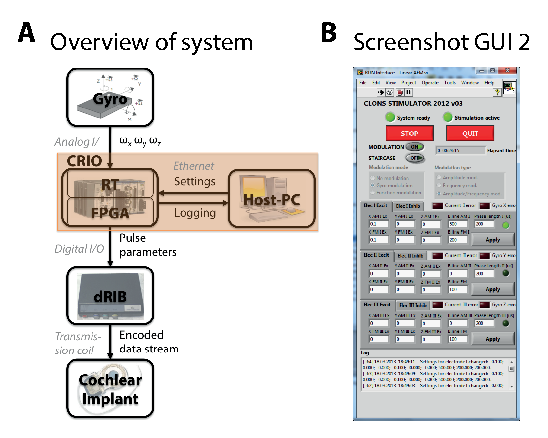
\includegraphics{chapters/partii/crio/figures/Fig_CRIO_overview.eps} 
\caption[CompactRIO system overview and user interface]{System overview and user interface. (\textbf{A}) From top: A gyroscope senses rotation and is connected to the analog input interface of the CompactRIO (CRIO). It features a real-time (RT) controller and a field programmable gate array (FPGA). The RT controller exchanges data with a host-PC via ethernet. RT, FPGA and PC (orange block) constitute the core of the system. Parameters are sent digitally from the FPGA to the direct Research Interface Box (dRIB) that translates them into MED-EL’s proprietary data stream. The stream is sent through a transmission coil to the cochlear-vestibular implant that generates the appropriate stimulation pulses. (\textbf{B}) The main interface (GUI 2) during stimulation. The operator starts and stops the stimulation, selects modulation mode and type (PAM, PRM, PAM/PRM), and specifies gains and baselines for the three controlled electrode sites. A log at the bottom displays the events.}
\label{fig:crio:overview}
\end{figure}
	
\subsection{Hardware}
\subparagraph{Gyroscope}
A wearable unit containing a MEMS gyroscope has been developed for the experiments with implanted patients (Carpaneto et al., 2015). The sensor was a 3-axis gyroscope (LYPR540AH by ST Microelectronics, Geneva, Switzerland) capable of measuring yaw, pitch and roll. 

Anti-aliasing filters were added, and the PCB with all components was encased in a 44x75x11\,mm metal box. A titanium screw on one side of the box allows for transcutaneous fixation to a subject’s mastoid. A \SI{2}{\metre} long cable carries the three angular rates, and two other lines for DC power supply (two AA batteries for safety reasons).

\subparagraph{CompactRIO (CRIO)}
We opted for National Instruments’ CRIO platform (NI, Austin, TX, USA) as research tool for several reasons: (i) powerful embedded controller; (ii) integrated FPGA for digital communication; (iii) LabVIEW’s ease to program GUIs; and (iv) compliance with safety standards and directives (IEC 61010, IEC 60601-1).

	Specifically, we assembled a system with the NI cRIO-9113 chassis (Virtex 5 FPGA), CRIO-9022 embedded controller, one NI\,9205 analog input module, three NI 9401 digital input/output modules, and the power supply module NI-PS 15. The Virtex-5 LX50 FPGA had 48 multipliers and 28’800 flip-flops, the embedded controller a \SI{533}{\mega\hertz} CPU, \SI{2}{\giga\byte} solid-state storage and \SI{256}{\mega\byte} DRAM. Both CPU and FPGA were mid-range performance components recommended by NI for our scenario. The analog input module NI\,9205 with 250'000 samples per second was sufficiently fast for three input channels (sampling period of up to \SI{12}{\micro\second}). The digital module NI\,9401 had a fast update rate of \SI{100}{\nano\second} to facilitate the communication between the FPGA and dRIB. A 34-pin flat ribbon cable for 16 data, three address, one enable, and ready bits connected the three modules with the dRIB. Data was transmitted when ready was set low by the dRIB; then the CRIO pulled the enable signal low for at least \SI{300}{\nano\second}. The whole system weighed \SI{2.3}{\kilogram}.
	
\subparagraph{Direct Research Interface Box (dRIB)}
Generally, Med-El implants convert a digitally encoded data stream to stimulation pulses. The format of this data stream is proprietary. Therefore, a device was needed to translate pulse properties -— such as pulse amplitude, phase duration, controlled electrode site —- into that stream with low latency. Current research tools for Med-El implants could not be used due to load-dependent response times of about \SI{200}{\milli\second} with large jitter (unpublished).
We built the dRIB on the basis of a previous device for Med-El implants (RIB1) that contained a microprocessor and a FPGA section for data encoding (Baumann and Nobbe 2006). Disabling the internal microprocessor allowed for an external 16-bit input that would send stimulation parameters from the CRIO. Additionally, a level shifter and boot-time disconnection logic were built and added to translate between the different logic levels of the CRIO and the dRIB. The dRIB provided lowest possible latencies: from completely written pulse data to pulse output 21x\SI{1.67}{\micro\second} = \SI{35}{\micro\second} (16 data bits, 3 address and 2 read/write bits at a transfer rate of \SI{600}{\kilo\hertz} from dRIB to implant). The interface box also guaranteed that only valid data was transmitted and ensured continuous power supply for the implant without specific knowledge of the data format.

\subparagraph{Personal computer (PC)}
All PCs used to program the CRIO ran Windows 7 (Microsoft Corporation, Redmond, WA, USA) and had LabVIEW 2011 with the RT and FPGA modules installed (National Instruments). PC CPU speed was not critical for performance. A LAN port was required to connect to the CRIO.

\subsection{Software}
Four different GUIs were implemented in LabVIEW: (i) a GUI with controls for configuration and monitoring; (ii) a GUI with stimulation settings; (iii) a GUI for RT processing and (iv) a GUI to monitor outgoing communication from the FPGA.

	These GUIs are specifically designed for the different hardware levels. GUIs 1 and 2 are executed on the PC, GUI 3 on the RT controller and GUI 4 on the FPGA. Figure\,\ref{fig:crio:interconnections} shows the interconnection of the CRIO components and the GUIs, Fig.\,\ref{fig:crio:flowcharts} illustrates the flow charts of GUIs 3 and 4.
	
\subparagraph{GUI 1: controls for configuration and monitoring}
This GUI has five tabs and is the main interface before start of stimulation. The first tab includes charts of angular velocities, pulse rates and pulse amplitudes. The second tab loads gyroscope calibration values and sets a phase delay (to delay acting on processed gyro input values, e.\,g. to mimic the time constant of the semicircular canals). Calibration values map the gyroscope coordinate system to the patient’s reference frame (DiGiovanna et al., 2012). The third tab specifies controlled electrode sites, current ranges (four ranges with 128 steps: 150, 300, 600, 1200 current units, 1\,cu equals approximately \SI{1}{\micro\ampere} and implant types (PULSAR/SONATA implant for clinical trials and benchmark tests or C40+ implant for benchmark tests only). The operator chooses a location where to save log files with the fourth tab. The final tab sets sinusoidal modulation of pulse amplitude and pulse rate.

\subparagraph{GUI 2: stimulation settings}
This GUI is most relevant for the operator during stimulation and its design was shaped by feedback from two clinicians and two engineers (Fig.\,\ref{fig:crio:overview}B). It features START/PAUSE and QUIT buttons. The operator selects between modes ‘No modulation’, ‘Gyro modulation’, or ‘Function modulation’, and between types ‘Amplitude modulation’ (PAM), ‘Rate modulation’ (PRM), or ‘Amplitude/Rate modulation’ (PAM/PRM). Two other controls toggle modulation and the staircase function (described further below). 

	Three panels set gains, phase length (length of cathodic and anodic phase, respectively), baseline pulse amplitude and pulse rate for each of the three electrode sites. Depending on the operating type, non-relevant control parameters are disabled. Furthermore, the operator is able to choose between symmetric or non-symmetric stimulation. Choosing the former, gains were identical for positive and negative angular velocities; choosing the latter allowed the operator to specify another set of gain values for negative angular velocities, effectively resulting in a piecewise linear transfer function. More advanced functions may be loaded in future software versions. 
	
	A log displays events such as start of stimulation and warnings. Each entry triggered a digital output for synchronization with video recordings and post-hoc analysis.
	
\subparagraph{GUI 3: real-time controller}
This GUI is deployed to CRIO’s embedded controller and has an empty graphical interface, since any interactive item would affect RT performance. The algorithm has two parts: a time-critical loop with high priority and a non-critical loop with lower priority. The non-critical loop runs every \SI{200}{\milli\second} and is responsible for data exchange between both GUIs 1 and 2 (on PC) and the GUI 3 on the embedded controller. Specifically, undeterministic network variables are copied to deterministic RT equivalents for use in the time-critical loop. The loop time of \SI{200}{\milli\second} was chosen to transfer stimulation parameters to the PC for logging as often as possible but without over-burdening the embedded controller with variable conversion.

	The time-critical loop processes incoming gyroscope voltages and calculates stimulation parameters; it runs every \SI{2}{\milli\second}. The conversion from voltages to angular velocities involves a 3x3 matrix multiplication with the three voltages. Pulse amplitude and pulse rate are calculated according to Eqs.\,\eqref{eq:crio1}-\eqref{eq:crio4} depending on operating mode and type. Pulse parameters are then sent to GUI 4. In principle this loop should run as often as possible. However, the execution time was \SI{1.2}{\milli\second}; thus the loop time had to be set to the next full millisecond (\SI{2}{\milli\second}) to comply with LabVIEW’s Timed Loops.

\subparagraph{GUI 4: FPGA}
This GUI is responsible for input and output communication. Upon start it initializes the dRIB. Then it periodically acquires and buffers gyro voltages (16-bit ADC) every millisecond. Each electrode site has a loop that writes stimulation parameters into a FIFO buffer at the time point specified by the pulse frequencies. For instance at 100 pulses per second (pps), the loop executes every \SI{10}{\milli\second} and writes the parameters for one stimulation pulse into the FIFO.

Due to the structure of these write loops, a special mechanism is implemented for low pulse frequencies less than 40\,pps. For example with 10\,pps, the loop would run only every \SI{100} {\milli\second} and write a pulse to the FIFO buffer. With PAM this does not pose a problem. However with PRM, this would prevent swift changes of pulse rates. Therefore, the mechanism checks every \SI{25}{\milli\second} whether the pulse rate has increased beyond 40\,pps and replaces the old stimulation pulse parameters with new ones if necessary. This gives priority to pulses with higher pulse rate. The 40\,pps threshold was an educated guess, and can be tuned by the operator.

Another part of the FPGA code checks the FIFOs every \SI{0.5}{\milli\second} and arbitrates in case pulses are scheduled simultaneously. Priority is given to the pulse with the highest pulse rate. If pulses have identical rates, output on electrode I comes before electrode II that comes before electrode III. The dRIB and the cochlear implant are not capable of activating electrode sites simultaneously (instead the next site would be activated \SI{0.5}{\milli\second} later).
GUI 4 is usually hidden and provides operators with advanced options such as overriding input signals.
\begin{figure}[btp]
\centering

\includegraphics{chapters/partii/crio/figures/Fig_CRIO_interconnection.eps} 
\caption[CompactRIO interconnection and signal flow]{Interconnections and signal flow between components. From top: Analog voltages for yaw, pitch and roll are digitized (NI9205) and buffered with GUI 4 on the FPGA as fixed point variables (fxp). Via the PCI bus, the values are read from GUI 3 running on the RT controller to compute current amplitude and pulse rate (floating point). Parameters are sent through Ethernet from the host PC (GUIs 1, 2) and have to be converted to deterministic RT variables. Stimulation values are then transmitted in GUI 4 through the three NI\,9401. A flat ribbon cable that has 16 data, 3 address and two control bits (enable, ready) connects the digital modules with the dRIB.}
\label{fig:crio:interconnections}
\end{figure}
\begin{figure}[btp]
\centering
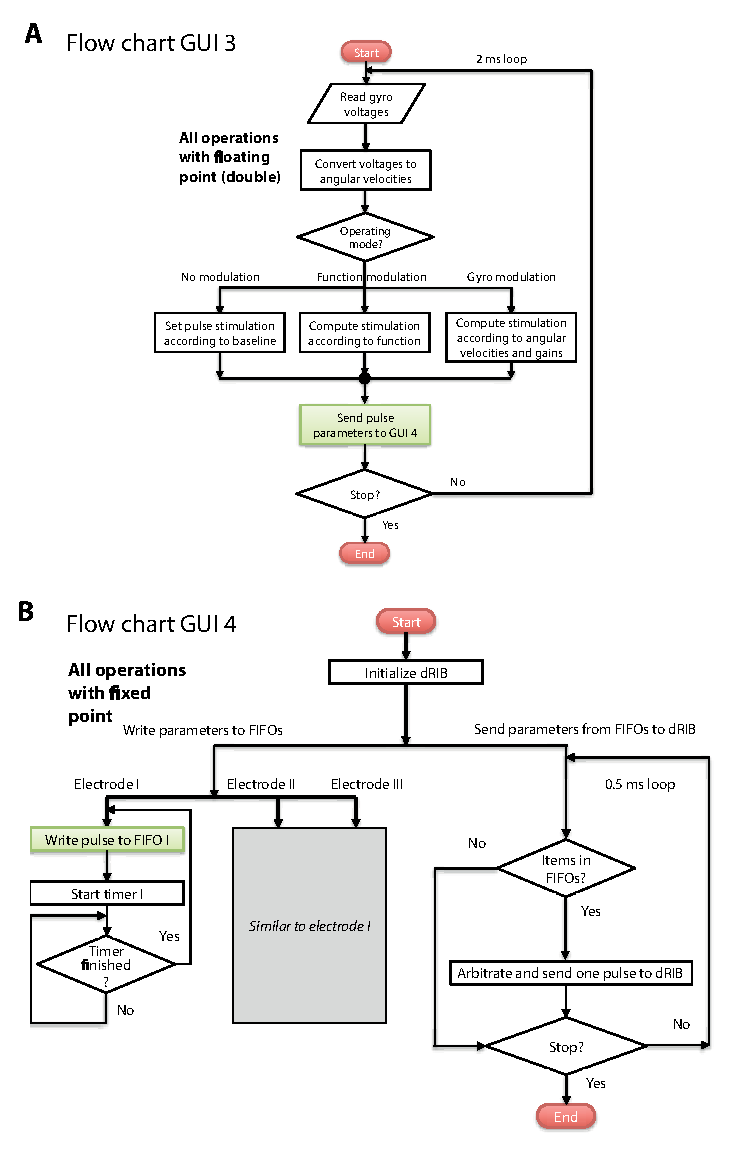
\includegraphics[height=.8\textheight]{chapters/partii/crio/figures/Fig_CRIO_flowchart.eps} 
\caption[CompactRIO flow charts for GUIs 3, 4]{Flow charts of GUIs 3 and 4. All operations in GUI 3 are done with floating point, in GUI 4 with fixed point. (\textbf{A}) The time-critical loop of GUI 3 starts with reading gyroscope voltages and converts them to angular velocities. Pulse parameters are then computed depending on the operating mode and sent to GUI 4 (green shaded box). The distinction between PAM, PRM and PAM/PRM is done inside the computation boxes and was excluded here for legibility. Commands are repeated every 2\,ms. (\textbf{B}) GUI 4 for the FPGA runs code extensively in parallel. After initialization of the dRIB, pulse parameters -- received from GUI 3 (green shaded box) -- are written into FIFOs for each electrode.  Timers are run to create a certain pulse rate (e.\,g., a timer of 10\,ms for 100\,pps). Simultaneously, another loop checks every 0.5\,ms whether the FIFOs are filled and sends out existing pulses to the dRIB giving priority to the pulse with the highest pulse rate.}
\label{fig:crio:flowcharts}
\end{figure}

\subsection{Implementation of operating modes and types}
This section elaborates on the various modulation modes. It also explains the inherent difficulty of implementing PRM using current cochlear implant technology. All gain and baseline parameters are taken from the GUIs 1 and 2.

\subparagraph{Mode ‘No modulation’}
This mode provides steady-state stimulation at the specified baseline pulse amplitudes and baseline pulse rates. In PAM mode, baseline pulse rates are identical for all three electrodes, and different baseline pulse amplitudes can be set. In PRM or PAM/PRM mode, each electrode has its own set of baseline values for both pulse amplitude and pulse rate.

	In this mode the staircase function is activated per default. It adapts subjects slowly to baseline stimulation as a sudden change in stimulation amplitude would be perceived as an abrupt change in head rotation and may result in severe symptoms such as nystagmus, vertigo and nausea. It increases current amplitude by 50\,cu every \SI{100}{\milli\second}, while pulse rate remains constant at baseline level. Vice versa, when stimulation is turned off, pulse amplitude is decreased by the same ratio.
	
\subparagraph{Mode ‘Function modulation’}
This mode modulates pulse amplitude and/or pulse rate according to a sinusoidal function regardless of gyro inputs (i.e., no patient movement required). Theoretically, modulation frequencies of up to \SI{500}{\hertz} are possible, but frequencies up to \SI{8}{\hertz} are physiologically most relevant (Pozzo et al., 1990).
In PAM mode, the current amplitude is calculated as:
\begin{equation}\label{eq:crio1}
I_1 = R_A \sin \left( 2\pi f t \right) + b_{A_1}
\end{equation}
where $R_A$ is the modulation range  (identical for all electrode sites), $f$ the modulation frequency, $t$ the elapsed time since the start of function modulation, and $b_A$ the baseline pulse amplitude.

In PRM mode, the pulse frequency is determined as:
\begin{equation}\label{eq:crio2}
P_1 = R_P \sin \left( 2\pi f t \right) + b_{P_1}
\end{equation}
where $R_P$ is the modulation range for the pulse rate, and $b_P$ the baseline pulse rate. Selecting the mixed mode PAM/PRM combines Eqs.\,\eqref{eq:crio1} and \eqref{eq:crio2}.

\subparagraph{Mode ‘Gyro modulation’}
This mode modulates parameters depending on the baseline values, gains and measured angular velocities, i.\,e. it mimics the rotation-based modulation of the vestibular system.

With PAM, stimulation pulses have a fixed pulse rate and pulse amplitude is computed as:
\begin{equation}\label{eq:crio3}
I_1 = g_{A_{x_1}}\omega_x + g_{A_{y_1}}\omega_y + g_{A_{z_1}}\omega_z + b_{A_1}
\end{equation}
where $I$ is the current amplitude, $b_A$ the baseline amplitude, and $g_A$ the PAM gains for the three angular velocities $\omega_x$, $\omega_y$ and $\omega_z$. The suffix 1 indicates electrode site 1. Equations for sites 2 and 3 are similar, but with different gains and baseline values. The current amplitude $I$ and baseline amplitude $b_A$ had the unit [cu], the gains [cu/(\degree /s)], and angular velocities [\degree /s]. If non-symmetric stimulation is chosen, then gains have different values for non-negative and negative angular velocities. 

	With PRM, the pulse amplitude is fixed to the baseline pulse amplitude and pulse rates are modulated as:
\begin{equation}\label{eq:crio4}
P_1 = g_{P_{x_1}}\omega_x + g_{P_{y_1}}\omega_y + g_{P_{z_1}}\omega_z + b_{P_1}
\end{equation}
where $P$ is the pulse rate, $b_P$ the baseline pulse rate, and $g_P$ the PRM gains. Similar equations are in place for electrode sites 2 and 3. Again, a second set of gains can be specified for negative angular velocities. The units were [pps] for $P$ and $b_P$ and [pps/(\degree /s)] for the gains.
	The mixed mode PAM/PRM combines Eqs.\,\eqref{eq:crio3} and \eqref{eq:crio4}: modulating both pulse amplitude and pulse rate, which can be regarded as the superposition of the two individual modes.
	
\subparagraph{Remarks on pulse rate modulation with cochlear implants}
Cochlear implants employ PAM as primary means to provide cues for speech recognition. Therefore, it can be directly implemented via interfacing with the dRIB registers for stimulation amplitude. However, there is no dRIB register to specifically set the pulse rate of each electrode site separately. Instead stimulation pulses are sent from CRIO to dRIB at appropriate fixed intervals to render baseline pulse rate.

	Due to the lack of a pulse rate generator in the dRIB, PRM can only be emulated on the CRIO with the limitations explained below. Given the code structure of GUI 4, pulses are transmitted at most every \SI{0.5}{\milli\second}, resulting in intervals of 2, 2.5, \SI{3}{\milli\second} etc. (minimum interval of \SI{2}{\milli\second}) equivalent to pulse frequencies of 500, 400, 333\,pps etc. Values like 450\,pps are achieved by switching between 500 and 400\,pps (i.\,e., pulse rate averaging). This creates a non-linear resolution of pulse rates with higher accuracy for lower pulse rates. This resolution is the most acceptable, given typical stimulation parameters. We decided to avoid shorter intervals, such as \SI{0.2}{\milli\second}, as they could result in a loss of pulses.

\subsection{Validation}

\subparagraph{Methods}
The following features were tested:
\begin{enumerate}
\item Response time (sensor input to stimulation output)
\item Mode: function modulation
\item Mode: gyro modulation
\item Phase delay
\end{enumerate}

To visualize stimulation pulses, a detector box acted as a substitute for a cochlear implant. A transmission coil from the dRIB was connected to a C40+ detector box for PAM and for PRM tests (Department of Ion Physics and Applied Physics at the University of Innsbruck, Innsbruck, Austria). It simulates a patient’s implant impedances with one resistor per electrode site. The PAM/PRM mode was validated with a PULSAR detector box (also University of Innsbruck). The two types of detector boxes differ slightly, the C40+ has a more non-linear current output (in amplitude). Both boxes had to be tested, since either could be used in clinical trials to monitor the output to the patient. In benchmark tests, stimulation pulses were recorded with a Tektronix MSO2014 (Tektronix, Beaverton, OR, USA) and Tektronix’ modified version of LabVIEW Signal Express 2011.

The response time was measured with voltage step inputs from 0.9 to \SI{2.3}{\volt}, representing a change of angular velocity from -700 to 950\,\degree /s. The steps were applied with frequencies from 0.25 to \SI{20}{\hertz} to cover a wide range of possible motion changes. (Frequencies of head movement in various locomotor tasks had harmonics up to \SI{8}{\hertz} or \SI{20}{\hertz} (Grossmann et al., 1988).) The step input was applied to one input channel, the other two channels were kept at \SI{0}{\volt}. Test inputs were generated with a TTi TG330 function generator (Thurlby Thandar Instruments, Huntingdon, UK).

Function modulation was tested in AM and FM modes for different modulation frequencies. The tested range of 200$\pm$150\,pps was typical for vestibular prosthesis prototypes (Merfeld et al., 2007). The PAM/PRM mode was validated in a single test covering the appropriate ranges in both modulation domains.
 
Sinusoidal voltage inputs for gyro modulation were generated with the TTi function generator. Additionally, a programmable phase delay was tested at \SI{50}{\milli\second}. All test parameters are listed in Table\,\ref{tab:crio1}.

\subparagraph{Analysis}
To assess performance we calculated latencies between the ideal output (reference signal) and the measured output. Root Mean Square Errors were computed with consideration of quantization errors (RMSE$_{\text{QE}}$). These are presented in the sections below. For reference we also report the RMSE$_{\text{ZQE}}$ assuming a zero quantization error, i.\,e., an ideal output device. All analysis was done in Matlab 2011a (MathWorks, Natick, MA, USA).
{\footnotesize
\begin{table}
\begin{threeparttable}[tbp]\footnotesize
\caption{Settings for CRIO validation}\label{tab:crio1}
\begin{tabularx}{\textwidth}{>{\centering\arraybackslash}m{.13\textwidth} >{\centering\arraybackslash}m{.13\textwidth} >{\centering\arraybackslash}m{.13\textwidth} >{\centering\arraybackslash}m{.13\textwidth} >{\centering\arraybackslash}m{.13\textwidth} >{\centering\arraybackslash}m{.13\textwidth}}
\toprule
Function mod. & Baseline pulse amplitude [cu] & Baseline pulse rate [pps] & Range & Mod. freq. [Hz] & \\
\midrule
PAM & 500 & 500 & 400\,cu & 2; 5 & \\
PRM & 500 & 200 & 300\,pps & 2; 5 & \\
PAM/PRM & 300 & 200 & 400\,cu & 2 & \\
& & & 300\,pps & &\\
\bottomrule
\toprule
Gyro mod. & Baseline amplitude [cu] & Baseline pulse rate [pps] & Gain & Phase delay [ms] & Input freq. [Hz]\\
\midrule
PAM & 500 & 500 & 0.1\,cu/(\degree /s) & 0 & 2; 5 \\
PAM & 500 & 500 & 0.1\,cu/(\degree /s) & 50 & 2 \\
PRM & 500 & 500 & 0.1\,cu/(\degree /s) & 0 & 2; 5 \\
PRM & 500 & 500 & 0.1\,cu/(\degree /s) & 50 & 2 \\
\bottomrule
\end{tabularx}
\begin{tablenotes}
\item Note: 500\,pps represents a worst-case load; 200\,pps represents a reasonable baseline pulse rate. We could not test worst-case in PRM as it would not have been possible to up-modulate.
\end{tablenotes}
\end{threeparttable}
\end{table}
}
\section{Results}
\subsection{Response time}
Figure\,\ref{fig:crio:response} shows response times at 200 and 500\,pps to a voltage step from 0.9 to \SI{2.3}{\volt} (equivalent to -700 to 950\,\degree /s). The step had a frequency of \SI{5}{\hertz}; the system was in gyro modulation mode PAM. One hundred measurements were taken. At 200\,pps, response times for rising and falling edges averaged at \SI{6.8}{\milli\second}, standard deviation was \SI{1.6}{\milli\second}, and the maximum latency was \SI{9.95}{\milli\second}. At 500\,pps, values were 5.2, 0.8, and \SI{6.6}{\milli\second}, respectively. The lower variance for the higher pulse frequency was also reflected in the histogram, where 40\% of samples were between 4.5 and \SI{5.5}{\milli\second} in contrast to 16\% for 200\,pps. Other step frequencies between 0.25 and \SI{20}{\hertz} did not significantly change results.
\begin{figure}[btp]
\centering
\includegraphics{chapters/partii/crio/figures/Fig_CRIO_response.eps} 
\caption[CompactRIO response times]{Response time. (\textbf{A}) At 200\,pps, the system responded to a step input (black trace) with a range of latencies from 4 to 10\,ms. (\textbf{B}) At 500\,pps, the range is smaller from 4 to 6.5\,ms, showing that response time was affected by baseline pulse rate. (\textbf{C}) and (\textbf{D}) show the histograms of response time for the two different conditions (total occurrences 100 each). At 200\,pps, response times were more widely distributed. In contrast, at 500\,pps, 40\% of response times were within 4.5 and 5.5\,ms.}
\label{fig:crio:response}
\end{figure}

\subparagraph{Mode ‘Function modulation’}
Pulse amplitude and/or rate were modulated as described in Eqs.\,\eqref{eq:crio1} and \eqref{eq:crio1}. Figure\,\ref{fig:crio:funcmod} shows function modulation for 2 and \SI{5}{\hertz} modulation frequencies. PAM function modulation demonstrated only small lags (2.3 and \SI{0.4}{\milli\second} positive peak lag and 1.7 and \SI{0.1}{\milli\second} negative peak lag). RMSE$_{\text{QE}}$ was zero (considering the quantization error of $\pm$13.4\,cu, i.\,e. the implant has limited pulse amplitude resolution), see Table\,\ref{tab:crio2}. 

In PRM mode, modulation range was 150\,pps at a baseline pulse rate of 200\,pps. Pulse rate steps were starkly noticeable at low frequencies. At high pulse frequencies, pulse rates had higher variance. The positive peak lags were 4.0 and \SI{1.5}{\milli\second} for 2 and \SI{5}{\hertz}; the negative peak lags 7 and \SI{-4.5}{\milli\second}, respectively. RMSE$_{\text{QE}}$ were less than 5\,pps (2.5\% of baseline). 

Figure\,\ref{fig:crio:funcmod}E, F depicts PAM/PRM at \SI{2}{\hertz} modulation frequency. In contrast to the other plots, parameters were slightly different and these traces were not averaged since only a single 2 second trial was included. The lags were small: \SI{3.5}{\milli\second} for the positive peak and \SI{0.0}{\milli\second} for the negative peak (PAM), \SI{-16.5}{\milli\second} and \SI{0.0}{\milli\second} for PRM. RMSE$_{\text{QE}}$ values were 0\,cu and 9.2\,pps (0 and 4.6\% of baseline, respectively).

\begin{figure}[btp]
\centering
\includegraphics{chapters/partii/crio/figures/Fig_CRIO_funcmod.eps} 
\caption[CompactRIO function modulation]{Validation of function modulation. (\textbf{A}) Modulation of pulse amplitude at 2\,Hz and 200\,cu magnitude at 500\,cu baseline. (\textbf{B}) Modulation at 5\,Hz. In both cases, the averaged measured output (blue) agreed with the reference (green band) showing RMSE$_{\textbf{QE}}$ of zero (accounting for quantization error). (\textbf{C}) and (\textbf{D}) show modulation of pulse rate at 2 and 5\,Hz. The black lines in PRM plots illustrate the exact reference, while the green band illustrates the margin of error due to the non-linear pulse rate resolution. RMSE$_{\textbf{QE}}$ was 1.4\,pps for 2\,Hz and 3.4\,pps for 5\,Hz. At low pulse rates the limited resolution became clearly visible. (\textbf{E}) and (\textbf{F}) represent a single trial (not averaged) of the combined PAM/PRM mode. The trial lasted 2 seconds, and the plots show the first 0.5\,s to match subplots A-D. RMSE$_{\textbf{QE}}$ were 0\,cu and 9.2\,pps. All lags are summarized in Table\,\ref{tab:crio2}.}
\label{fig:crio:funcmod}
\end{figure}

{\footnotesize
\begin{table}
\begin{threeparttable}[tbp]\footnotesize
\caption{Statistics for CRIO function modulation}\label{tab:crio2}
\begin{tabularx}{\textwidth}{>{\centering\arraybackslash}m{.16\textwidth} >{\centering\arraybackslash}m{.16\textwidth} >{\centering\arraybackslash}m{.16\textwidth} >{\centering\arraybackslash}m{.16\textwidth} >{\centering\arraybackslash}m{.16\textwidth}}
\toprule
Test & Lag pos. peak [ms] & Lag neg. peak [ms] & RMSE$_{\text{QE}}$ & RMSE$_{\text{ZQE}}$  \\
\midrule
PAM 2\,Hz & 2.3 & 1.7 & 0\,cu (0\%) & 5.1\,cu (1.0\%) \\
PAM 5\,Hz & 0.4 & 0.1 & 0\,cu (0\%) & 4.1\,cu (0.8\%) \\
PRM 2\,Hz & 4.0 & 7 & 1.4\,pps (0.7\%) & 8.8\,pps (4.4\%) \\
PRM 5\,Hz & 1.5 & -4.5 & 3.9\,pps (2\%) & 10.7\,pps (5.4\%) \\
PAM/PRM: PAM & 3.5 & 0.0 & 0\,cu (0\%) & 4.2\,cu (1.4\%)\\
PAM/PRM: PRM & -16.5 & 0.0 & 9.2\,pps (4.6\%) & 15.4\,pps (7.7\%)\\
\bottomrule
\end{tabularx}
\begin{tablenotes}
\item Lags and RMSE for individual PAM and PRM tests were calculated from averages, whereas the values for the combined PAM/PRM test were taken from a 2 second single trial. Two RMSE values were computed to account for the quantization error RMSE$_{\text{QE}}$ and to compare it to an ideal output with zero quantization error RMSE$_{\text{ZQE}}$, i.e. the reference signal had zero tolerance. RMSE values in brackets are in percent of baseline.
\end{tablenotes}
\end{threeparttable}
\end{table}
}
{\footnotesize
\begin{table}[tbp]\footnotesize
\caption{Statistics for CRIO gyroscope modulation}\label{tab:crio3}
\begin{tabularx}{\textwidth}{>{\centering\arraybackslash}m{.16\textwidth} >{\centering\arraybackslash}m{.16\textwidth} >{\centering\arraybackslash}m{.16\textwidth} >{\centering\arraybackslash}m{.16\textwidth} >{\centering\arraybackslash}m{.16\textwidth}}
\toprule
Test & Lag pos. peak [ms] & Lag neg. peak [ms] & RMSE$_{\text{QE}}$ & RMSE$_{\text{ZQE}}$  \\
\midrule
PAM 2\,Hz, 0\,ms & 5.5 & 1.4 & 0\,cu (0\%) & 5.8\,cu (1.2\%) \\
PAM 2\,Hz, 50\,ms & 4.2 & 0 & 0\,cu (0\%) & 6.9\,cu (1.4\%) \\
PAM 5\,Hz, 0\,ms & 2 & 2.4 & 0\,cu (0\%) & 5.3\,cu (1.1\%) \\
PRM 2\,Hz, 0\,ms & 6.2 & 13.9 & 7.9\,pps (4\%) & 12.3\,cu (6.2\%) \\
PRM 2\,Hz, 50\,ms & 10.8 & 12.9 & 7.9\,pps (4\%) & 12.3\,cu (6.2\%) \\
PRM 5\,Hz, 0\,ms & 5.5 & 11.8 & 20.8\,pps (10.4\%) & 27.6\,cu (13.8\%) \\
\bottomrule
\end{tabularx}
\end{table}
}
\subparagraph{Mode ‘Gyro modulation’}
The main objective of the new system was to couple modulation of the stimulation signal to a 3-axis gyroscope sensor in real-time (we had tested function modulation in humans before). Validation results are depicted in Fig.\,\ref{fig:crio:gyromod}. The top row shows PAM, the bottom row PRM for one output channel. Tests not reported herein with all input and output channels active showed correspondingly similar results.

	Due to the function generator's DC settings, the input was slightly unsymmetrical peaking at -750 and +1000\,\degree /s. Measurements were averaged over 50 samples for 2\,Hz and 100 for 5\,Hz. A reference signal was calculated from the input signal $\omega_x$, and a gain of 0.1\,cu/(\degree /s) for $g_{A_{x_1}}$ PAM or 0.1\,pps/(\degree /s) for $g_{P_{x_1}}$ PRM (cf. Eqs.\,\eqref{eq:crio3}-\eqref{eq:crio4}). All other gains were zero. The graphs in the left and right columns had no phase delay, the center column had a \SI{50}{\milli\second} phase delay. 

In PAM, the measured output followed the reference. Differences were less than the quantization error. The positive peaks of input and output lagged \SI{5.5}{\milli\second} for \SI{2}{\hertz} sinusoidal input and \SI{0}{\milli\second} delay, \SI{4.2}{\milli\second} for \SI{50}{\milli\second} phase delay, and \SI{2}{\milli\second} for \SI{5}{\hertz} and \SI{0}{\milli\second} delay. The lags for the negative peak were 1.4, 0.06, and \SI{2.4}{\milli\second}, respectively. These statistics and RMSE$_{\text{QE}}$ equaling zero are summarized in Table\,\ref{tab:crio3}. 

In PRM, the baseline pulse rate was 200\,pps. Two main observations were made. First, a high variance of pulse rate was recorded for pulse rates above 250\,pps. Second, the output lagged the reference more for negative than positive angular velocities (13.9 vs \SI{6.9}{\milli\second} for \SI{2}{\hertz}, \SI{0}{\milli\second} delay). The latencies for other scenarios did not exceed \SI{13}{\milli\second} and are shown in Table\,\ref{tab:crio3}. RMSE$_{\text{QE}}$ was about 7.9\,pps for both \SI{2}{\hertz} cases and 20.8\,pps for \SI{5}{\hertz} stimulation (4 and 10.4\% of baseline pulse rate, respectively).

\begin{figure}[btp]
\centering
\includegraphics[width=.98\textwidth]{chapters/partii/crio/figures/Fig_CRIO_gyromod.eps} 
\caption[CompactRIO gyroscope modulation]{Validation of gyro modulation. PAM (\textbf{A-C}) and PRM (\textbf{D-F}). (\textbf{A}) Baseline pulse amplitude was 500\,cu and baseline pulse rate 500\,pps. The black trace illustrates averaged input angular velocity, the green band the desired output signal and blue trace the averaged output. The input signal had a frequency of 2\,Hz and no input delay. RMSE$_{\text{QE}}$ was 0\,cu. (\textbf{B}) Same as (A) but with an input delay of 50\,ms (vertical dashed lines). Reference and measured output shifted accordingly and RMSE$_{\text{QE}}$ was 0\,cu. (\textbf{C}) A higher input frequency of 5\,Hz did not affect the output signal and remained within the reference. (\textbf{D}) Baseline pulse rate was 200\,pps. The averaged measured output followed the reference, but showed large variance at high pulse rates and a visible lag at low pulse rates. The lag for the positive peak was 6.2\,ms, for the negative peak 13.2\,ms. RMSE$_{\text{QE}}$ was 7.9\,pps (4\% of baseline rate). (\textbf{E}) Same as (D) but with 50 ms input delay depicted by the two black dashed lines. Output was also delayed by 50\,ms. RMSE$_{\text{QE}}$ was very similar to (D). (\textbf{F}) At a higher input frequency of 5\,Hz, RMSE$_{\text{QE}}$ increased to 20.8\,pps, while lags were comparable to (D) and (E).}
\label{fig:crio:gyromod}
\end{figure}

\section{Discussion}
Our system's primary design constraint was that the latency between acquiring angular velocities and modulating stimulation output should not exceed \SI{6.5}{\milli\second}.	The performance of our system remained below or close to the limit; all modulation modes were accurate. These diverse modes have previously shown effects on eye movement responses in animal models (Davidovics et al., 2012, 2013). With our system we will be able to evaluate which paradigm is optimal in humans; this insight will be critical for design of future portable vestibular prosthetics.

\subparagraph{System architecture}
Vestibular prostheses for animal models have employed tailored circuits typically with microcontrollers (Gong and Merfeld, 2000; Fridman and Della Santina, 2012), or alternatively with CMOS technology (Constandinou et al., 2008), or with a field-programmable analog array (Toreyin and Bhatti 2013). These low-cost systems can provide faster response times, but translation to clinical studies in patients has remained difficult. The use of modified, commercially available, cochlear implants offers a fast-track to a vestibular implants in humans since it is based on established and medically certified technology. Our system with a modified implant is not portable, but is intended as research platform and provides clinicians with flexibility to study stimulation paradigms and parameters. Additionally, some restrictions applied due to interfacing the proprietary implant software (forced through the dRIB). These aspects should be regarded as confounds when comparing the CRIO system with others.

	Two groups have tested modified cochlear implants in rhesus monkeys: one based on a Concerto MED-EL implant (Valentin et al., 2013), the other one on Nucleus Freedom implant (Cochlear Corporation) (Phillips et al., 2011; Nie et al., 2013). The former had a belt-worn unit with a Bluetooth interface to tune parameters and a head-worn unit with a gyroscope and radio frequency link to the implanted stimulator. The system was portable. Similar to our approach, their software used a ‘time-until-next-pulse’ to create pulse rate stimulation. For the modulation, parameters were determined with a 32 bin look-up table (Valentin et al., 2013), whereas our system performed floating point calculation. Regarding the other implant, a setup with a research processor applied various pulse trains (similar to our function modulation) (Nie et al., 2013); for real-time processing (gyro modulation) one had to switch to another setup with a clinical processor (Phillips et al., 2011). The CRIO can transition between function and gyro modulation seamlessly.
	
	These other systems delivered in-vivo results consistent with earlier work of those groups. However, they did not report response times, or elaborate on implementing pulse rate modulation with cochlear implant technology.
	
\subparagraph{Response time}
At 200\,pps baseline pulse rate, our average response time from sensor input to stimulation output was \SI{6.8}{\milli\second} with a standard deviation of \SI{1.6}{\milli\second}. At 500\,pps, the values were 5.2 and \SI{0.8}{\milli\second}. Latencies from pulse train stimulation to eye movement in cats were measured at \SI{3.8}{\milli\second} (200\,pps) or \SI{3.5}{\milli\second} (500\,pps) (Cohen and Suzuki 1969). Latencies to single pulses were timed at 5-6\,ms in cats (Cohen and Suzuki 1969) or squirrel monkeys (Merfeld et al., 2007). Therefore, the total response time from sensor input to eye movement onset with our system can be stated as 10.6$\pm$\SI{1.6}{\milli\second} for 200\,pps or 8.7$\pm$\SI{0.8}{\milli\second} for 500\,pps. These would be within the range of natural response times (7.5$\pm$2.9, 7.6$\pm$2.8, and 10.3$\pm$\SI{1.9}{\milli\second} for yaw, pitch and roll, respectively (Aw et al., 1996)). Though our system would be slightly slower for two axes, the VOR has demonstrated high adaptability. For instance, VOR gains and phase as well as alignment improved with chronic stimulation (Lewis et al., 2002; Dai et al., 2011). These findings suggest that the VOR response could adapt to the suboptimal CRIO stimulation. Additionally, the impact of a slower response time could be studied with the ‘phase lag’ parameter.

The maximum CRIO latency observed at 200\,pps was \SI{9.95}{\milli\second}. Theoretically, the maximum response time was \SI{10.5}{\milli\second}, composed of \SI{4}{\milli\second} to read and process an input change, 3x\SI{0.5}{\milli\second} to send pulse parameters for three electrodes and \SI{5}{\milli\second} for the pulse period at 200\,pps (\SI{4}{\milli\second} + 3x\SI{0.5}{\milli\second} + 1/200\,pps). Reading and processing were performed in GUI 3, the output of pulse parameters in GUI 4. Likewise at 500\,pps, we observed a maximum latency of \SI{6.62}{\milli\second}, the highest theoretical value was \SI{7.5}{\milli\second}. The response time could be reduced by activating only one electrode site and thus lowering the number of calculations and writing operations. This could halve the processing time (time-critical loop of GUI 3) and the maximum time from input to stimulation output at 200\,pps would be \SI{4.5}{\milli\second} (\SI{2}{\milli\second} + 1x\SI{0.5}{\milli\second} + 1/200\,pps). A similar improvement could be achieved with a stronger processor than \SI{533}{\mega\hertz}. These improvements will be implemented if clinical tests prove them to be necessary. 

Pulse rate influenced latencies. The higher the pulse rate, the sooner an updated pulse could be applied. The 200\,pps baseline pulse rate, that was tested agrees with the common approach in unilateral implants to use a higher than normal baseline pulse rate to evoke both excitatory and inhibitory eye movement responses. Human subjects have been adapted to baseline pulse frequencies of 200\,pps (Guyot et al., 2011a) and 400\,pps (unpublished). Therefore we do not expect to operate at a baseline with slower response times than those reported herein.

\subparagraph{Mode ‘Function modulation’}
This mode was primarily designed to characterize eye movement responses to PAM, PRM or PAM/PRM. A sinusoid was chosen, because it is a smooth function without abrupt changes that could lead to patient discomfort. 

Function modulation of PAM was fast and accurate. Quantization error could have been reduced, by selecting a smaller current range. The tradeoff would be a lower maximum output level. 
Function modulation of PRM was also accurate. Due to the non-linear pulse frequency resolution (500, 400, 333\,pps etc.), any value between resolution steps was rendered on average through fast switching between adjacent pulse rates (e.\,g., Fig.\,\ref{fig:crio:funcmod}C at \SI{150}{\milli\second} shows the averaged pulse rate switching between 333 and 400\,pps). At lower pulse rates, switching was slower because of the resulting lower update rate. For instance at 77\,pps, the next change of pulse rate was applied \SI{13}{\milli\second} later (1/77\,pps). This lower update rate explains the negative peak lags of \SI{7}{\milli\second} for \SI{2}{\hertz} and \SI{-4.5}{\milli\second} for \SI{5}{\hertz} (e.\,g., steps in Fig.\,\ref{fig:crio:funcmod}C,D). In the former case, the lowest pulse rate was in effect after the negative peak, whereas in the other case it occurred before. Therefore, the main contributor to RMSE$_{\text{QE}}$ was the lower update rate, particularly below 100\,pps.

\subparagraph{Mode ‘Gyro modulation’}
Gyro modulation performed well. In contrast to function modulation, gyro modulation was less jagged. Specifically for PRM, it did not show the clear pulse rate steps present with function modulation (Fig.\,\ref{fig:crio:gyromod}F vs. Fig.\,\ref{fig:crio:funcmod}D). This was due to response time jitter. For instance, the onset of the smallest pulse rate output had a standard deviation of \SI{4.7}{\milli\second} for FM \SI{5}{\hertz} in gyro modulation mode compared to \SI{0.3}{\milli\second} in function modulation mode. This small variance effectively smoothed the average responses in Fig.\,\ref{fig:crio:gyromod}.

Latencies for positive and negative peaks for PAM were below the crucial threshold of \SI{6.5}{\milli\second}. This was partly true for the positive peak lag with PRM, results for the negative peak lag were larger than \SI{10}{\milli\second} and can be attributed to the lower update rate present at pulse rates below 100\,pps.

The phase delay in PAM and PRM mode moved the output accordingly by the specified \SI{50}{\milli\second}, and otherwise did not change the characteristics of the signal. The delay could be used to better fit electrically evoked responses with natural VOR responses (arising from sensors with a known time constant).

The frequency of the input signal did not influence PAM output, RMSE$_{\text{QE}}$ was zero. In PRM mode, however, the \SI{5}{\hertz} input frequency yielded lags like the \SI{2}{\hertz} case (high lags at low pulse rates), and consequently led to more than twice as high RMSE$_{\text{QE}}$. The errors for 5 and \SI{2}{\hertz} had a ratio of 2.6 (5/2 equaling 2.5).  

RMSE$_{\text{QE}}$ for gyro modulation PRM were larger than for function modulation. For \SI{2}{\hertz} function modulation it was 1.4\,pps, for gyro modulation 7.9\,pps. The error at lower pulse rates was exacerbated by the response time to the gyroscopic input which was disregarded during function modulation, illustrated by larger negative peak lags (7 vs. \SI{13.9}{\milli\second}).

\subparagraph{Comparing PAM, PRM and PAM/PRM}
PAM, PRM, and PAM/PRM modulations are ready for operation. A thorough study is required to determine the most effective and efficient modulation paradigm in humans. Previous studies on a human patient showed that PAM elicited slightly stronger eye movements than PRM, but both modes were not systematically compared and parametric changes were not exhaustive (Guyot et al., 2011).

One advantage of PRM may be lower current spread than with PAM. PRM alone has shown less misa-lignment of VOR in chinchillas (Davidovics et al., 2012) and rhesus monkeys with modified cochlear implants (Nie et al., 2013). The underlying hypothesis was that the total number of evoked action potentials influenced VOR. This number can be changed (in PAM) through recruiting more neurons with a higher pulse amplitude (thus increasing the risk of current spread), or (in PRM) by making already recruited neurons fire more often with a higher pulse rate. 

However with PRM mode, two issues warrant highlighting: first, the non-linear pulse rate resolution, especially at high pulse rates, and second, the lower update periods leading to an error with decreasing input signals. It has to be noted, that the tested angular velocities were extremely high (-750 to 1000\,\degree /s) and more than twice the value experienced with head impulse tests (Cremer et al., 1998) and much higher than angular velocities recorded during healthy locomotion that peaked at 140\,\degree/s (Pozzo et al., 1995). Subjects with vestibular disorders are expected to experience lower angular velocities for activities such as running in light or darkness (Pozzo et al., 1991).

Regarding the first issue, it will be interesting to see whether subjects will be able to notice the fast switching between pulse rates like 222.2 and 250\,pps. It is important to stress that these are instantaneous rates. Future perceptual tests should clarify the exact meaning of the PRM RMSE. Specifically, we will verify whether pulse rate is estimated by the vestibular system instantaneously (i.e. dt between the current and prior pulse) or in a longer history of multiple pulses through averaging, If the latter case held, this would effectively smooth the errors calculated herein.

The second issue will likely result in lower than expected inhibitory eye movement responses or asymmetry between excitatory and inhibitory responses; a problem witnessed with unilateral implants and physiological baseline stimulation rate that was not alleviated with chronic stimulation (Dai et al., 2011). Elevated baseline pulse rate evoked more symmetrical responses (Merfeld et al., 2007). That option and the possibility to set different gains for positive and negative angular velocities should be explored to produce symmetric eye movement responses. Bilateral implantation is another approach (Gong et al., 2008), but remains unlikely in humans due to the inherent risks of two surgeries.

The combination of PAM and PRM could also improve responses. Both could complement each other. It has been shown that co-modulation increased the range of eye movement responses (Davidocis et al., 2012, 2013). The authors suggested using co-modulation to provide a wide range of excitatory and inhibitory responses with a unilateral implant. However, this effect has yet to be shown in humans.

\section{Summary}
We presented a system that can interface a 3-axis gyroscope sensor with a custom MED-EL cochlear-vestibular implant and is capable of modulating three independent stimulation outputs to angular velocities with a latency similar to natural VOR latency. The system offers tools for pulse amplitude and pulse rate modulation as well as a combination thereof. A second advantage is the computational power allowing for floating point calculation and for more complex transfer functions. Graphical user interfaces are the third main advantage letting the operator change parameters with ease while stimulation is active without the need to pause the stimulation (a critical feature to avoid nystagmus). 

	Patient trials with the system are ongoing and have focused first on the characterization of eye movement responses to function modulation of PAM and PRM. The outcome of these experiments is described in the following Chapter\,\ref{chap:pamprm}.
